\documentclass{ltjbook}
\usepackage{docmute} 
\usepackage{../../myStyle} 

\begin{document}
\chapter{実験計画法3；一要因モデル(Within)}
\label{m14_design3}

ここまで，線形モデルとしての実験計画法を見てきました。一要因，二要因がそれぞれ単回帰分析，\keytermL{重回帰分析}{じゅうかいきぶんせき}に対応すること，二要因以上になると組み合わせの効果が出現することなどを見てきました。
しかしここまでの話はいずれも，\keytermL{群間要因}{ぐんかんよういん}計画の話でした。そこで\keytermL{群内要因}{ぐんないよういん}計画の場合はどのようになるか，というところに目を向けていきたいと思います。
\section{Within計画の場合}
群内要因での例を考えていくにあたって，今回も数値例を基に話を始めてから，線形モデルでの表現へ，と進めていきたいと思います。

今回は一要因3水準の，群内計画の要因計画の話をしましょう。データに対応がある，あるいは反復測定であることがポイントです。同じ人に複数回データを提供してもらう，次のような状況をイメージしてください。

臨床心理学者がある介入法をつかってメンタルケアに取り組んでいます。4人のクライアントにこの手法を適用し，抑うつ度が改善されていくかどうかチェックします。表\ref{tbl::22_05}のようなスコアが得られたとき，この介入法に効果あるかどうかを考えたい，とします。
% latex table generated in R 4.0.2 by xtable 1.8-4 package
% Fri Sep 11 14:57:29 2020
\begin{table}[ht]
	\centering
	\caption{Within Data Example}
	\begin{tabular}{lrrr}
		\hline
		ID & Time1 & Time2 & Time3 \\
		\hline
		1  & 10    & 5     & 9     \\
		2  & 9     & 4     & 5     \\
		3  & 4     & 2     & 3     \\
		4  & 7     & 3     & 5     \\
		\hline
	\end{tabular}
	\label{tbl::22_05}
\end{table}
このデータを図にしてみましょう。ポイントは，3つの調査時点(Time1,2,3)それぞれが独立ではなく，クライアント番号(ID)は共通しているというところです。横軸は時間だとすると，その軸に意味がありますから，同じ人のデータ点を線で結ぶことができるのです。

\begin{figure}
	\centering
	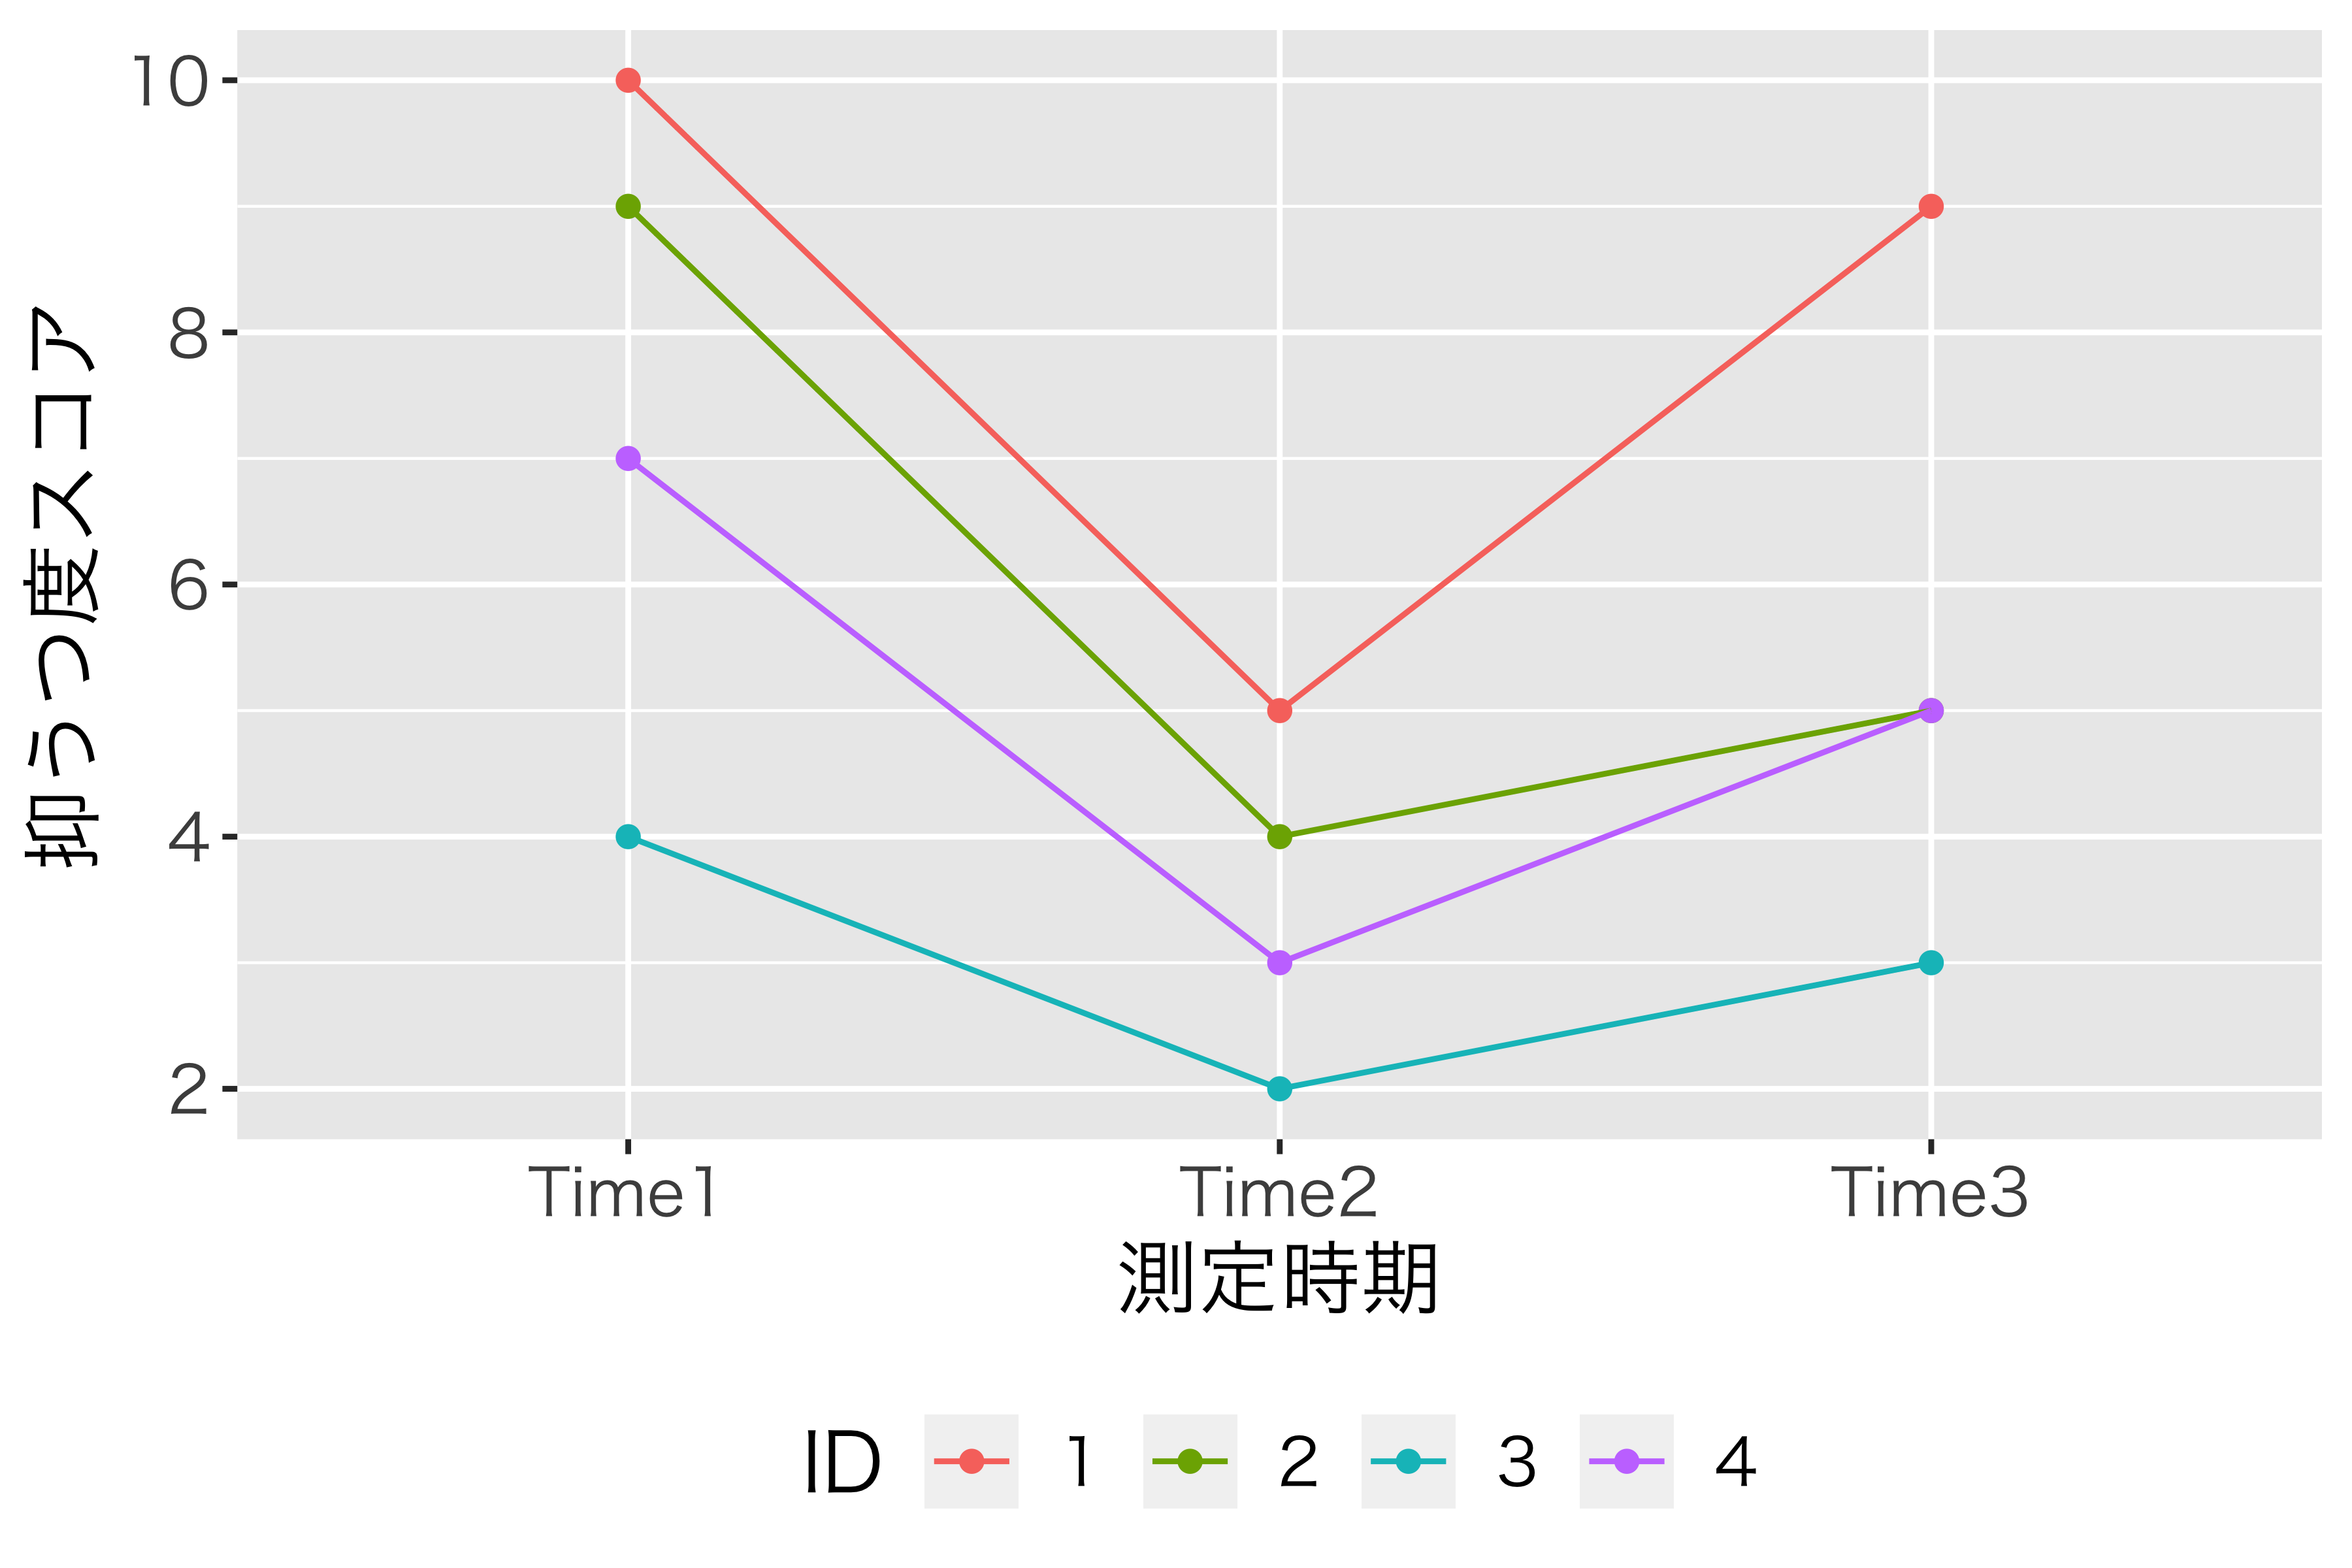
\includegraphics[keepaspectratio,width=8cm]{../images/22_anovaOnR/Rplot22_03.png}
	\caption{介入効果によるクライアントの状態変化}
	\label{fig::22_05}
\end{figure}
図\ref{fig::22_05}をみていると，個人差こそあれ，第一期(Time1)から二期(Time2)にかけては一旦下降傾向があり，第二期から三期(Time3)にかけては上昇傾向があるのかなあ，と思ったりします。この直感をデータで検証してくことが大事ですね。

ここで考えたいのは，「個人差こそあれ」のところです。\keytermL{個人差}{こじんさ}があるというのは，最初10点から始まるのか(ID=1)，4点から始まるのか(ID=3)，というところで既に7点差ついてるのですが，今回これは個人差であって見たい効果の部分ではない，と考えるということです。見たい効果は「時期」要因による，3つの水準それぞれへの影響，$b_j$ です。数式的に表現すると，個人$i$ の第$j$期におけるデータ$y_{ij}$は，次のように表すことができます。

\[ y_{ij} = b_0 + d_i + b_j X_{ij} + e_{ij} \]

ここで$X_{ij}$はまたしても，第$j$期に$b_j$の効果がある($1$)かない($0$)かを表している記号だと思ってください。具体的には，$i$さんの3つの時期$j=1,2,3$の効果を隠さずに書くとしたら，次のようになっていることに注意です。
\begin{equation}
	\begin{array}{ll}
		y_{i1} & = b_0 + d_i + b_1 X_{i1} + b_2 X_{i2} + b_3 X_{i3} + e_{i1}       \\
		       & = b_0 + d_i + b_1 \times 1 + b_2 \times 0 + b_3 \times 0 + e_{i1} \\
		       & = b_0 + d_i + b_1 + e_{i1}                                        \\
		y_{i2} & = b_0 + d_i + b_1 X_{i1} + b_2 X_{i2} + b_3 X_{i3} + e_{i2}       \\
		       & = b_0 + d_i + b_1 \times 0 + b_2 \times 1 + b_3 \times 0 + e_{i2} \\
		       & = b_0 + d_i + b_2 + e_{i2}                                        \\
		y_{i3}
		       & = b_0 + d_i + b_1 X_{i1} + b_2 X_{i2} + b_3 X_{i3} + e_{i3}       \\
		       & = b_0 + d_i + b_1 \times 0 + b_2 \times 0 + b_3 \times 1 + e_{i3} \\
		       & = b_0 + d_i + b_3 + e_{i3}                                        \\
	\end{array}
\end{equation}

また，ポイントとして，新たに$d_i$というのが出てきていることに注意してください。これは$i$に伴って変わる数字で，時期$j$の添字がついていませんから，「時期を通して一貫した個人の平均値」ということになります。$b_0$は$i$も$j$もついていませんから，個人にも時期にも関係なく変化しない全体の平均値を表しています。

\begin{figure}[ht]
	\centering
	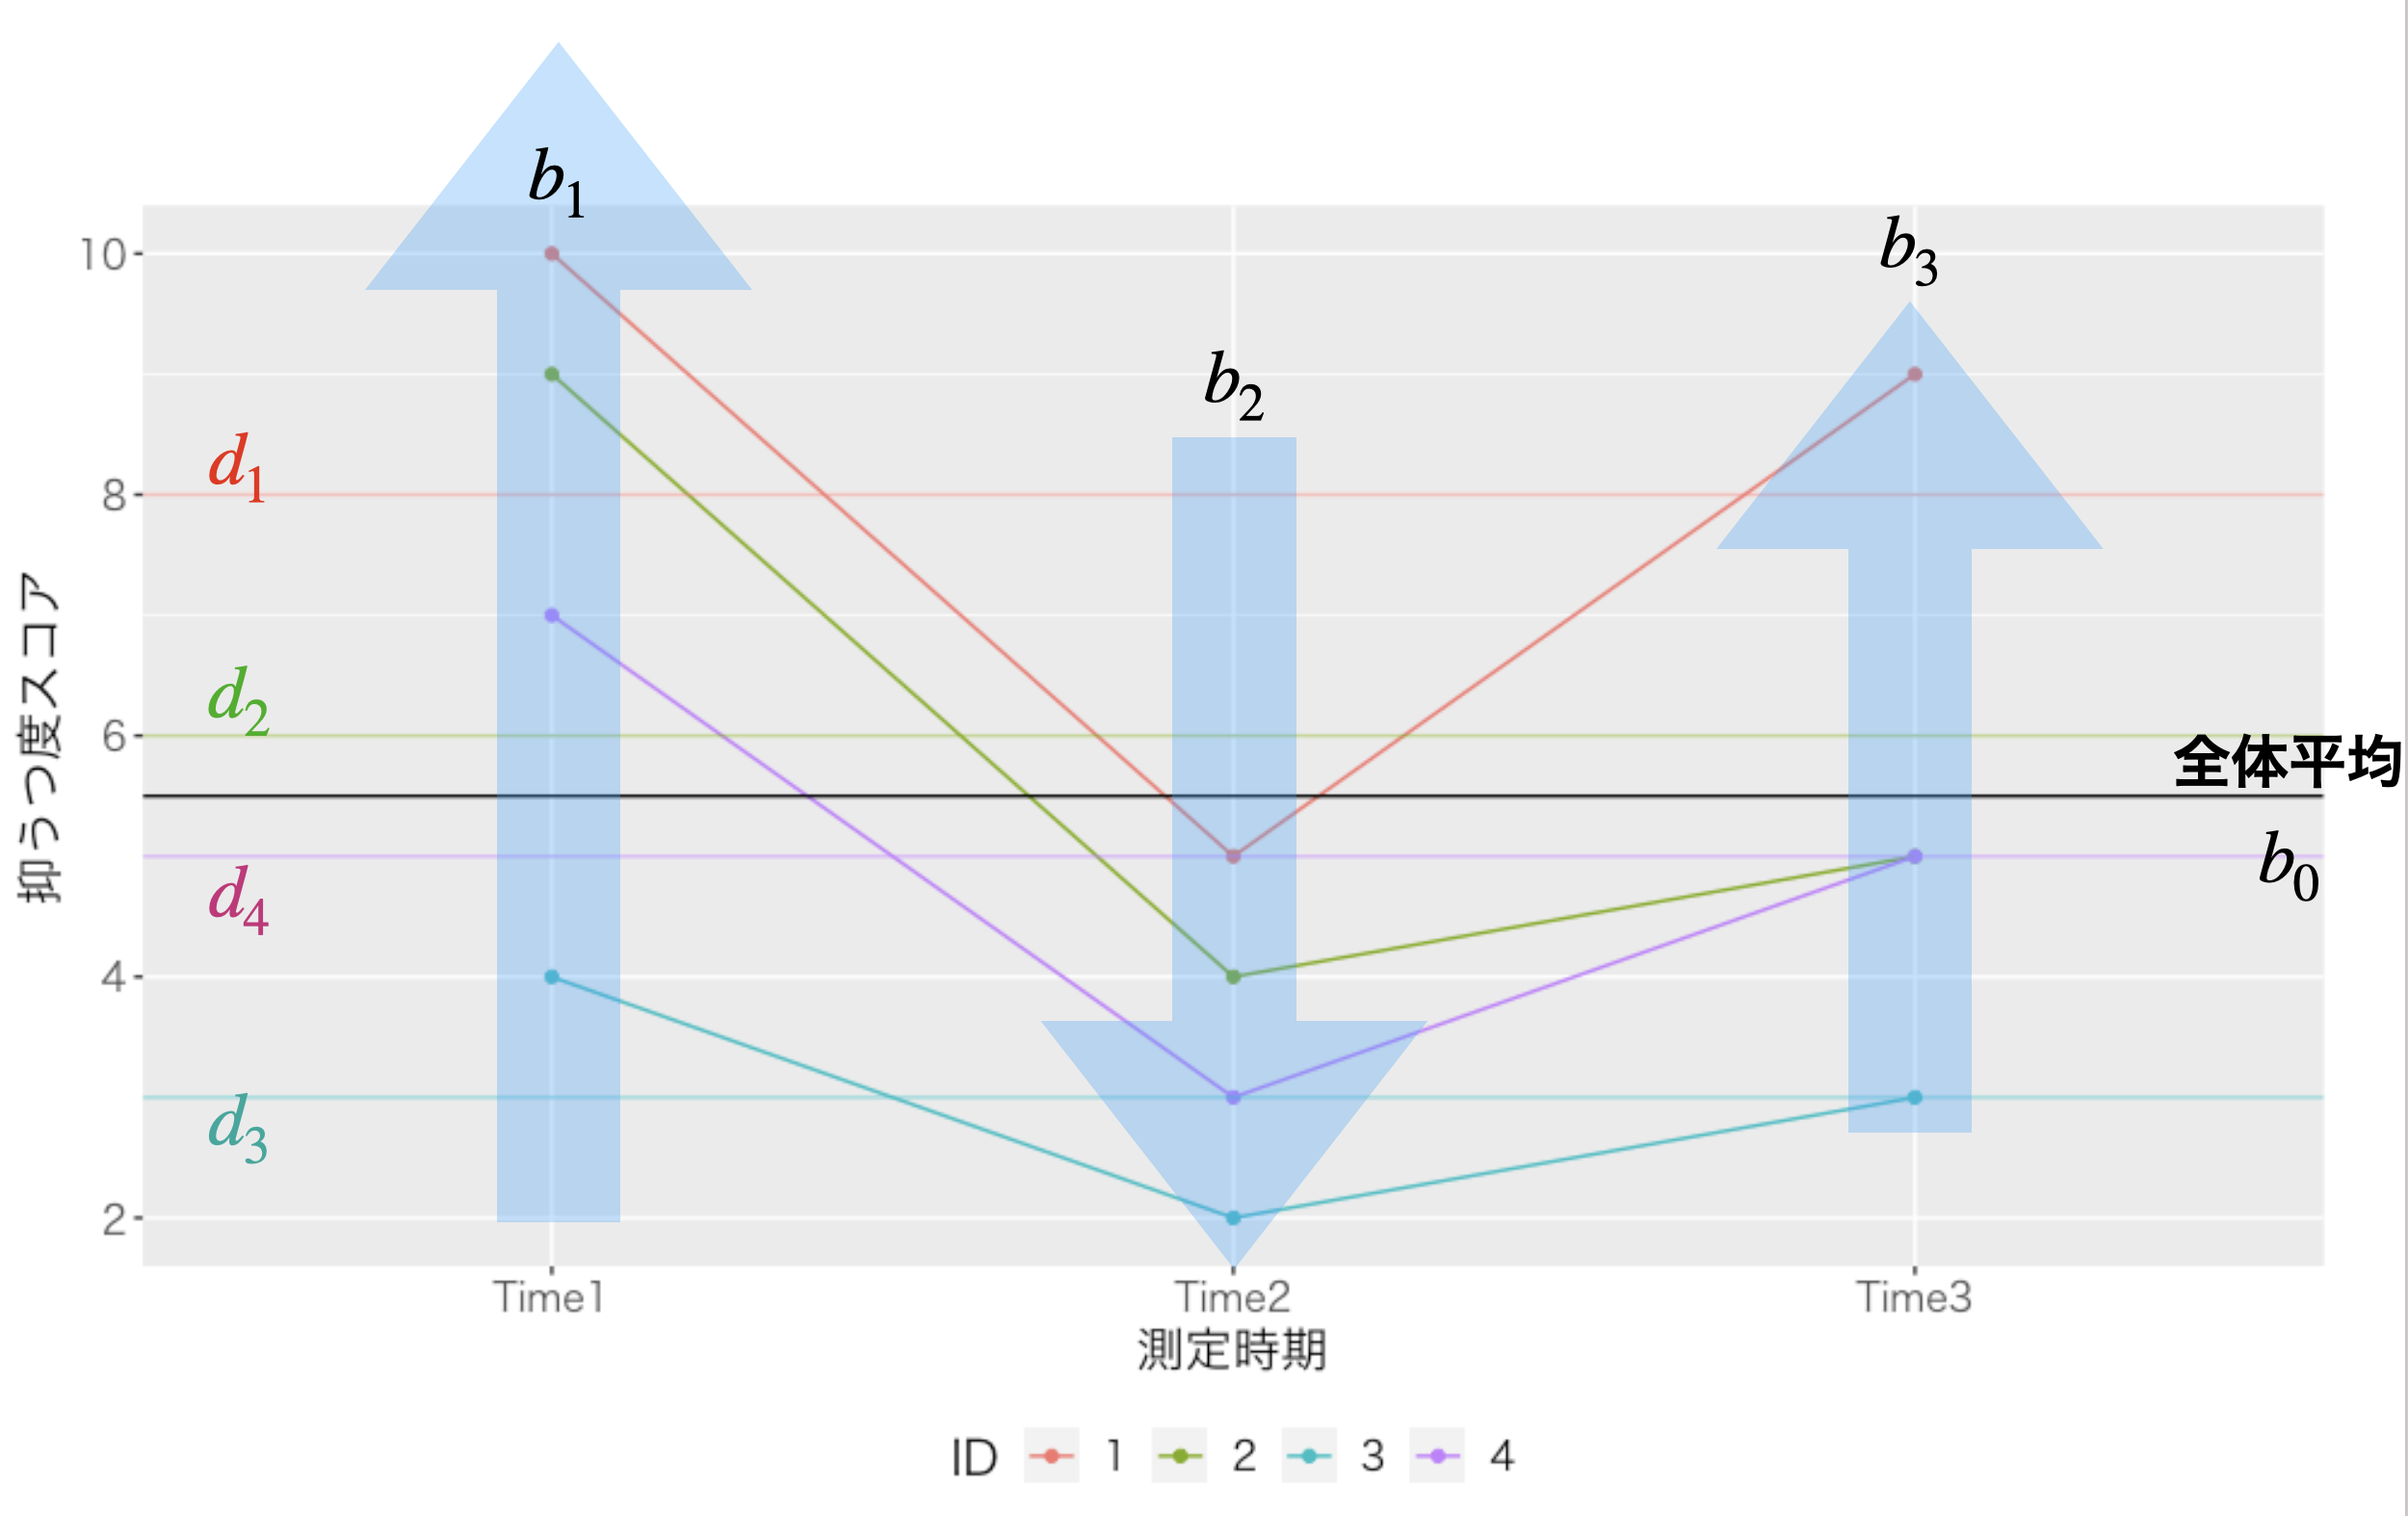
\includegraphics[keepaspectratio,width=12cm]{../images/14_design3/slide14_01.png}
	\caption{線形モデルで表現}
	\label{fig::22_06}
\end{figure}

これを図で表したのが図\ref{fig::22_06}です。全体平均$b_0$とは別に，個別の平均$d_i$の水平線が引かれています。個人平均は個々人のベースラインですので，時期によって変わりません。時期の効果$b_j$は4人に等しく影響します。添字$i$がないことでこれを表現しています。効果は同じであったとしても，個人の平均が違うので，データとして得られる数字は様々になっている，というわけです。もちろん個人差，効果を考慮しても析出できない誤差$e_{ij}$がありますし，これまで同様$b_{j}$は相対的，つまり全ての水準を足し合わせると$0$になってしまうものです。また，個人の平均値$d_i$も相対的なものとして捉えられます。全体平均$b_0$が別にあるからですね。これまで同様に無作為に割り付けているので，何の効果も個人差もなかったら，全体平均の横一線に並ぶはずだ，というのが基本的なアイデアだからです。

具体的な数字を使って考えてみましょう。表\ref{tbl::22_05}の行平均，列平均，全体平均を計算してみました。
行方向の平均は個人ごとの平均です。最初の人(ID=1)は平均が$8$ですから，全体平均から考えて$+2.5$の個人差がある人なのです。
また，列方向の平均は水準ごとの平均で，これが今回見たい効果ということになります。第1期(Time1)は平均が$7.5$ですから全体平均から考えて$+2.0$の効果があった時期だ，ということです。

個別のデータ，例えばID=1の第2期のデータは，理論通りに行けば，全体平均$5.5$に個人差$+2.5$と時期の効果$-2.0$が加わって出てくるはずです。$5.5+2.5-2.0＝6.0$になるはずですが，実際は$5$ですね。この違いは，理論では考えられないところなので，誤差になります。
% latex table generated in R 4.0.2 by xtable 1.8-4 package
% Fri Sep 11 14:57:29 2020
\begin{table}[ht]
	\centering
	\caption{水準ごとの平均から効果を考える}
	\begin{tabular}{lrrr|r}
		\hline
		ID   & Time1 & Time2 & Time3 & 平均 \\
		\hline
		1    & 10    & 5     & 9     & 8    \\
		2    & 9     & 4     & 5     & 6    \\
		3    & 4     & 2     & 3     & 3    \\
		4    & 7     & 3     & 5     & 5    \\
		\hline
		平均 & 7.5   & 3.5   & 5.5   & 5.5  \\\hline
	\end{tabular}
	\label{tbl::22_06}
\end{table}
こうして，効果，個人差，誤差を計算して表にしたのが表\ref{tbl::22_07}です。例によって総和すると0ですので，平方和を計算することで相対的な大きさを比較できるようになります。

% latex table generated in R 4.0.2 by xtable 1.8-4 package
% Fri Sep 11 15:52:17 2020
\begin{table}[ht]
	\centering
	\caption{効果，個人差，誤差を析出する}
	\begin{tabular}{llrcrrr}
		\hline
		ID     & 時期  & スコア & 全体平均 & 個人差 & 効果 & 誤差 \\
		\hline
		1      & Time1 & 10     & 5.5      & +2.5   & +2.0 & 0.0  \\
		1      & Time2 & 5      & 5.5      & +2.5   & -2.0 & -1.0 \\
		1      & Time3 & 9      & 5.5      & +2.5   & 0.0  & +1.0 \\
		2      & Time1 & 9      & 5.5      & +0.5   & +2.0 & +1.0 \\
		2      & Time2 & 4      & 5.5      & +0.5   & -2.0 & 0.0  \\
		2      & Time3 & 5      & 5.5      & +0.5   & 0.0  & -1.0 \\
		3      & Time1 & 4      & 5.5      & -2.5   & +2.0 & -1.0 \\
		3      & Time2 & 2      & 5.5      & -2.5   & -2.0 & +1.0 \\
		3      & Time3 & 3      & 5.5      & -2.5   & 0.0  & 0.0  \\
		4      & Time1 & 7      & 5.5      & -0.5   & +2.0 & 0.0  \\
		4      & Time2 & 3      & 5.5      & -0.5   & -2.0 & 0.0  \\
		4      & Time3 & 5      & 5.5      & -0.5   & 0.0  & 0.0  \\
		\hline\hline
		平方和 &       &        &          & 39.0   & 32.0 & 6.0  \\\hline
	\end{tabular}
	\label{tbl::22_07}
\end{table}

ここにあるように，個人$i$の時期$j$における誤差，と各セルに細かく誤差が計算できるようになりました。これが群内要因計画の強みなのです。

\section{群間計画と群内計画の比較}
ここで\keyterm{群間要因}{ぐんかんよういん}{Between Design}計画と\keyterm{群内要因}{ぐんないよういん}{Within Design}計画の構造的な違いに触れておきたいと思います。

群内計画では，個人が誰であるかという情報があったので個人差を算出でき，それに基づいて分析しました。
が，群内計画の時のデータを群間計画のように分析してみるとどうなるでしょうか。表\ref{tbl::22_06}にある数字が同じであれば，当然全体の平方和(分散)は同じです。ただ個人情報が抜けているのであれば，効果と誤差にしか分割できません。言い換えると，群間計画というのは誤差の中に個人差が含まれており，「これは誤差なのかな，個人差なのかな？ 」という区別がつかない状態である，ということです(図\ref{fig::22_07})。

最終的には，誤差の大きさに対して効果の大きさはどうか，という観点から評価します\footnote{統計的な評価，価値判断の方法については後期の推測統計学で扱うので，ここでは比較して考える要素が何であるかを理解していただければ十分です。}。効果の大きさ＝分子が同じデータであれば，分母が小さい方が相対的に大きいと判断されることになりますね。群間計画の時の誤差は偶然誤差と個人差を含んでおり，群内計画の時は個人差を含みませんから，\underline{群内計画の方が群間計画よりも，分析の精度が高い}ということになります。

であれば，全ての研究が群内計画であればよいのに，と思うかもしれません。ただし現実的な問題として，同じ人に何度も何度もデータを提供してもらうのは，非常に負担をかけることになります(群内計画は反復測定計画とも呼ばれるのでした)。研究倫理的な観点，あるいは計画上の手間を考えると，群間計画にせざるを得ないということが少なくありません。研究者，研究に協力してくれる人，のコストを考えて実験計画はデザインする必要があるということです。

\begin{figure}[ht]
	\centering
	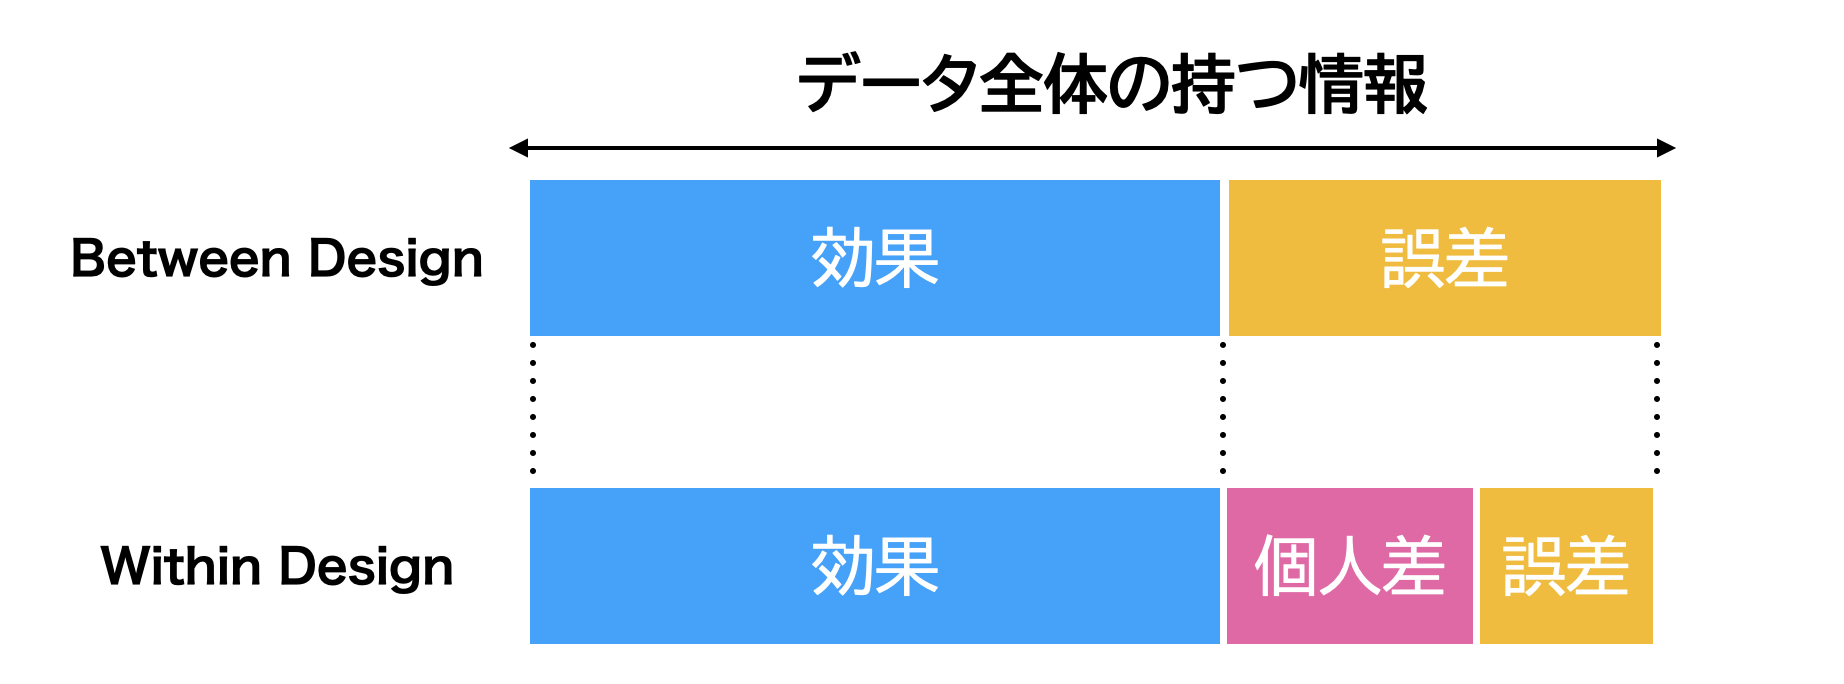
\includegraphics[keepaspectratio,width=12cm]{../images/22_anovaOnR/slide22_04.png}
	\caption{群内計画と群間計画の違い}
	\label{fig::22_07}
\end{figure}


\section{線形モデルによる表現と自由度}
\label{GeneralLinearModel}
さてこれまで，実験計画は説明変数が離散変数になっただけで，線形モデルの一種であるという説明をしてきました。
数学的な表現が苦手な人もいるかもしれませんが，$y=ax+b$，あるいは回帰分析の表現に則って$y=b_0 + b_1x$でもいいですが，要因計画も一次関数の特殊なパターンなのだという点を強調してきました。

なぜそのような流れで話をするかというと，回帰分析と要因計画は実は同じ\keytermL{モデル}{もでる}なんだよ，ということがわかると今度はそのモデルをこう変えたらどうなる？こっちのこれをいじったらどうなる？とどんどん発展させていくことができるからです。実際，心理学の研究で使われている分析は回帰分析系の子孫たちであり，今後これらを活用するために「要因計画で考えたら実質的にどういう違いを表しているのか」「線形モデルではどう表せるのか」と多角的なものの見方ができるようになってほしいからです。

その第一歩である，要因計画と線形モデルで一般的に\footnote{一般といわれると「ありふれていること」「広く行き渡っていること」を意味しているように聞こえますが，元々の意味は「同一である」というものです。他のものと同一，他のものを通じて変わらないもの，と思ってください。}説明できるということを表して，\keyterm{一般線形モデル}{いっぱんせんけいもでる}{General Linear  model}という言い方をします。
これを少し詳しく見てみましょう。

説明変数が連続変数である，いわゆる回帰分析モデルは，次のような式で表現されるのでした。
\[ y_i = b_0 + b_1 x_i + e_i \]

回帰分析の下になるのは相関関係ですから，変数$x_i,y_i$のいずれもx軸，y軸上のあらゆる値をとり得るものと考えられます。\keytermL{間隔尺度水準}{かんかくしゃくどすいじゅん}以上の数字で，説明変数が一単位増加したら，従属変数がどれぐらい増加するかを$b_1$で表しているのでした。

要因計画の場合は，説明変数が離散的です。離散的である，というのは尺度水準でいうと\keytermL{名義尺度水準}{めいぎしゃくどすいじゅん}にあるということです。
例えば統制群に1，実験群に2という数字を割り当てた，といった数値化をした時ですね。ただし1,2とコーディングしてしまうと，数式上は2の群が1の群の2倍という意味になるので，このままでは一般的に書くことができません。数学的にも成り立つし，実質的な意味としても通じるようなコーディングの仕方を考えましょう。

一番シンプルなのは，統制群を0，実験群を1とする方法です。例えばID=1の人を統制群としたら$x_1=0$ですし，ID=4の人が実験群であれば$x_4=1$である，と決めるのです。こうすると，統制群の回帰モデルは次のようになります。

\[ y_i = b_0 + b_1 \times 0 + e_i = b_0 + e_i \]
同様に，実験群の回帰式は次のようになります。

\[ y_i = b_0 + b_1 \times 1 + e_i = b_0 + b_1 + e_i \]

どちらの群も$b_0$がありますが，これは何も処置をしない群の平均値を意味します。統制群のデータの散らばりは，全て誤差$e_i$で説明するモデルということになります。

他方，実験群は，何もしない状態$b_0$に\textbf{加えて}$b_1$があり，それ以外の変化は誤差$e_i$で説明するということになります。ここで効果の大きさ$b_1$は添字$i$がついていないことを確認しましょう。効果の大きさは，個人ごとに変わるものではないからです。この$b_1$の総量が効果の大きさになりますが，比較すべき誤差$e_i$の総和はゼロになりますから，そのままでは比較せずに二乗して比較するようになります。

この表現の仕方は，統制群に比べて効果の大きさ$b_1$を見るというもので，比較的わかりやすい表現かと思います。でも水準数が3つになったらどう表したらいいのでしょうか。

大丈夫です，このときも基本的に考え方は変わりません。3つの群として前回の例，「水を毎日あげる」「水をときどきあげる」「水をあげない」とあったとしましょう。その上で，第一の群である「毎日水をあげる」群を基本に考えて式を立ててみましょう。

\[
	\begin{cases}
		y_{i1} = b_0 + e_{i1}       & \mbox{毎日水をあげる群} \\
		y_{i2} = b_0 + b_1 + e_{i2} & \mbox{ときどきあげる群} \\
		y_{i3} = b_0 + b_2 + e_{i3} & \mbox{あげない群}
	\end{cases}
\]

このようにすると，まず「水をあげる群」は$b_0+e_i$となっています。$e_i$は誤差・個体差を表しているので，この式は水をあげる群の各個体は，群平均と誤差からなるということを意味しています。
続いて第二の群ですが，式は$b_0 + b_1 + e_i$になりました。これは$b_0$すなわち水をあげる群の平均ですから，それに比べて「ときどき」群の平均が$b_1$だけ増え，さらに群内の個体差があるという順になります。あげない群も同様に，$b_0$に比べて$b_2$だけ平均が違う，ということになります。

しかしなぜ「水をあげる群」からスタートしたんでしょうね。あげない群と比べた方が，意味的にはわかりやすかったですかね。でも他のシーンで，A,B,C....X群とたくさんの水準がある時に，なぜ特定の群を基準にしたのだと言われても合理的な説明ができないかもしれません。

また要因計画では前提として，「群わけしなければ同じ状態だったもの」に「群わけ」という操作を加えて効果を算出しているのですから，原理的には分ける前の状態，すなわち全ての個体を1つの群としてみたときの状態が基本だったわけです。
ですから，その基本状態を$b_0$(全体平均)として，毎日水をあげる効果を$b_1$，時々あげる効果を$b_2$，あげない効果を$b_3$として，同様に考えてみましょう。

そうすると，3つの群のデータはそれぞれ次のように表現できることになります。

%amsmathパッケージ
\[
	\label{eq13_01}
	\begin{cases}
		y_{i} = b_0 + b_1 + e_{i} & \mbox{毎日水をあげる群} \\
		y_{i} = b_0 + b_2 + e_{i} & \mbox{ときどきあげる群} \\
		y_{i} = b_0 + b_3 + e_{i} & \mbox{あげない群}
	\end{cases}
\]

ここで$b_0$とあるのは，全体平均です。水のあげかたの違いになんの効果もなければ，全て全体平均＋個体差で説明できてしまうはずだからです。よろしいでしょうか。

このようにすると，一次関数の式のように，$X$を使った表現をしやすくなりました。ここで$X$は$X=\{0,1\}$でその項について「該当する/当てはまる/割り当てられている($1$)」か「該当しない/当てはまらない/割り当てられていない($0$)」かだけを意味するのだ，というルールにします。
例えば$i$番目のデータが「毎日水をあげる群」だったとすると，$X_{i1}=1,X_{i2}=0,X_{i3}=0$のように表します。すなわち，「水をあげる群」であり($1$)，「ときどきあげる群」「あげない群」ではない($0$)とするのです。これを踏まえて式を書き改めると，次のようになります。
\[
	\label{eq13_01b}
	\begin{cases}
		y_{i} = b_0 + b_1X_{i1} + b_2X_{i2} + b_3X_{i3} + e_{i} & \mbox{毎日水をあげる群} \\
		y_{i} = b_0 + b_1X_{i1} + b_2X_{i2} + b_3X_{i3} + e_{i} & \mbox{ときどきあげる群} \\
		y_{i} = b_0 + b_1X_{i1} + b_2X_{i2} + b_3X_{i3} + e_{i} & \mbox{あげない群}
	\end{cases}
\]

全て同じ式になってしまいました！どの群も$y_{i} = b_0 + b_1X_{i1} + b_2X_{i2} + b_3X_{i3} + e_i $という1つの式で表現できていますから，非常に簡略化できましたね。
またこうすると，群$j$のところが繰り返されていますから，$\sum$の記号を使って次のように書いてもいいかもしれません。

\[ y_i = b_0 + \sum_{j=1}^3 b_j X_{ij} + e_i \]

さらにさらに，$b_0$だけ表に出ているのが美しくないですね！ここで$X_{i0}=1$と決めてしまうと，さらにスマートに表現できます。

\[ y_i = \sum_{j=0}^3 b_j X_{ij} + e_i \]

うん，スッキリ。

ところでこれはちょっと余談ですが，数字をまとめて表現する，\keyterm{行列}{ぎょうれつ}{matrix form}による表現を使うと，もっと表現が楽になります。$i$番目のデータがどの群に割り当てられているかは，$\bm{X}_i = (1,0,0) $のように数字のセット，\keytermL{ベクトル}{べくとる}で表現されます。

ベクトルをセットで扱うのが\keytermL{行列}{ぎょうれつ}と呼ばれるもので，これを使うとデータセットは次のように表現できます。
\[
	\begin{pmatrix} y_1 \\ y_2 \\ \vdots \\ y_n \end{pmatrix}
	=
	\begin{pmatrix} b_0 \\ b_0 \\ \vdots \\ b_0 \end{pmatrix}
	+
	\begin{pmatrix} b_1 & 0 & 0 \\ 0 & b_2 & 0 \\ \vdots &\vdots & \vdots\\ 0 & 0 & b_3 \end{pmatrix}
	+
	\begin{pmatrix} e_1 \\ e_2 \\ \vdots \\ e_n \end{pmatrix}
\]
ここで右辺の第二項は$b_{ij}X_{ij}$の計算結果を表したもので，これを掛け算の式のまま表現すると，次のように書くことができます\footnote{行列とベクトルを習っていない人は，この掛け算どうなってるの？と思われるかもしれません。こうした行列の表現は線形代数と呼ばれるもので，心理統計のように変数が多くなったときの簡便的な表記法についての体系です。この授業の発展形である，データ解析応用の授業では行列を扱いますが，足し算掛け算から丁寧にやっていきますのでご心配なく。むしろ美しく表現できることにときめいてください。}。
\[
	\begin{pmatrix} y_1 \\ y_2 \\ \vdots \\ y_n \end{pmatrix}
	=
	\begin{pmatrix} 1 & 1 & 0 & 0 \\ 1 & 0 & 1 & 0 \\ \vdots  & \vdots & \vdots & \vdots \\ 1 & 0 & 0 & 1 \end{pmatrix}
	\begin{pmatrix} b_0 \\ b_1 \\ b_2 \\ b_3 \end{pmatrix}
	+
	\begin{pmatrix} e_1 \\ e_2 \\ \vdots \\ e_n \end{pmatrix}
\]

こうした上で行列やベクトルを記号で置き換えると，$\bm{y} = \bm{Xb} + \bm{e}$となり，このとき$\bm{X}$のことを(どの要因が割り当てられているかを表している行列という意味で)\keyterm{デザイン行列}{でざいんぎょうれつ}{design matrix}といいます。



さてここで式をよくみてください。2水準のときに比べると少し記号が増え過ぎな気がしませんか？ 統制群と実験群だけの2群のときは，統制群が$b_0$で実験群が$b_1$，計2つだけだったのですが，3水準になると$b_0,b_1,b_2,b_3$と4つの係数を考えることになっています。なぜ係数が3つで済まなかったのでしょう。

実はこの式には，ひとつ大事な\textbf{制約}が欠けているのです。全体平均からの相対的な大きさで効果を考える場合，「相対的」ですから全体平均を中心にしなければなりません。言い換えるならば，効果だけを足し合わせると総和が0になるような制約が必要なのです。これを式で表現すると次のようになります。

\[ b_1 + b_2 + b_3 = 0 \]

この式を展開すると次のようになります。
\[ b_3 = 0 - (b_1 + b_2) = -b_1 - b_2 \]
これを踏まえて式\ref{eq13_01}を書き直すと，次のようになります。

\[
	\label{eq13_02}
	\begin{cases}
		y_i = b_0 + b_1 + e_i       & \mbox{毎日水をあげる群} \\
		y_i = b_0 + b_2 + e_i       & \mbox{ときどきあげる群} \\
		y_i = b_0 - b_1 - b_2 + e_i & \mbox{あげない群}
	\end{cases}
\]

こうすると，モデル式の係数は$b_0,b_1,b_2$の3つになり，3水準で係数が3つなので計算が合いますね。
ちなみに2水準のときも全体平均を用いで表現するならば，次のようになります。

\[
	\begin{cases}
		y_i = b_0 + b_1 + e_i & \mbox{統制群} \\
		y_i = b_0 - b_1 + e_i & \mbox{実験群} \\
	\end{cases}
\]

このように表記すると，効果$b_1$の総和も0，誤差$e_i$の総和も0なので，二乗しないと計算できないなあということが理解しやすいかと思います。

ここで伝えたかったポイントは，「効果や誤差の大きさは相対的で，正負が同じ大きさだけ出るから足し合わせるとゼロになるから，大きさを評価するには二乗することで符号を消さなければならない」ということと，「効果の大きさを表す係数は，その要因の水準数$-1$個しか求められない」ということです。2つ目のポイントは特に，効果を評価するときに確率分布を応用する推測統計学の話に入ったとき，\keyterm{自由度}{じゆうど}{degrees of freedom}というパラメータに繋がる話なので，先走って解説しておきました。また第\ref{m21_anova}講あたりで出てくる話になりますので，それまで少し頭の片隅にでも引っ掛けておいていただければと思います。


\section{分布を使って考える}
\label{thinkWithDistribution}
さて，ここで前期の最後に少し発展的な要素も含んだお話をしておきましょう。

要因計画がどのようなものであれ，データの散らばりを生んでいるのは効果，個人差，偶然誤差によるものだと考えるのでした。逆に言えば，これらがなければ全ての値は同じになるはずだ，という観点から逆算し，効果，個人差，偶然誤差の大きさを見積もっていったのでした。

ここで，誤差を考える時には確率の考え方を利用してそれをコントロールする，という話を思い出してください。ガウスが考えた誤差論は，平均が$0$，分散$\sigma^2$で散らばる正規分布に従うのでした。すなわち誤差を$e_{i}$とすると，次のように表現できます。
\[ e_{i} \sim Normal(0, \sigma) \]


群間計画の場合は，各項目の値$y_i$を切片$b_0$と効果$b_1$と誤差に分けます。
\[ y_i = b_0 + b_1 + e_i \] \[e_i \sim Normal(0, \sigma) \]

数式の中に図を入れるのは御法度かもしれませんが，イメージでいうなら次のような形です。
\begin{figure}[h]
	\centering
	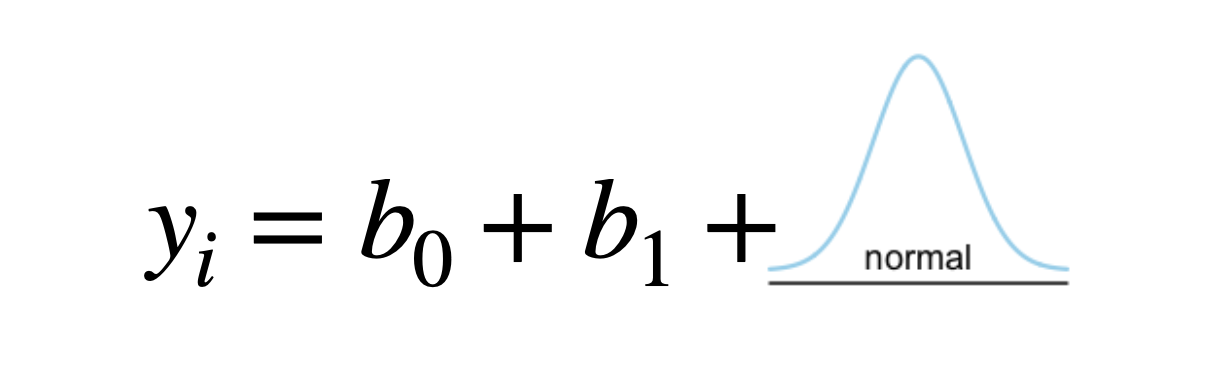
\includegraphics[keepaspectratio,width=6cm]{../images/14_design3/slide14_02.png}
\end{figure}

$e_i$が正規分布に従うのですが，$b_0+b_1$のところは確率的に変わるものではないことに注意してください。ここが確率的に変わらないということをよく考えれば，数式に沿ってある値が足されることと同じです。確率分布にある数字を加えると，その分布の位置がずれますね。正規分布は位置と幅でその特徴が作られているのですが，右辺全体で見ると，$b_0+b_1$のところは，正規分布の位置をずらすことでもあります。

ずれた分布は，正規分布の平均値が$b_0+b_1$ですから，式全体を整えると次のようになります。

\[ y_i \sim Normal(b_0+b_1 , \sigma) \]

この式のポイントは，$y=$ではなく$y\sim$になっているところです。データが正規分布に従う，という形に変わったのです。
線形モデル(要因計画)はこのように，\textbf{確率分布の位置パラメータに数式(モデル)を当てはめる}こととも言えます。

さらにさらに。
群内計画の場合は，個人差$d_i$も計算できるのでした。この個人差というのも，たくさん集めると確率的な傾向を表してくるはずで，特に個々人の生得的な性質に関係するのであれば，それはまた正規分布に従うと言えるでしょう。今回の個人差も相対的に捉えるので，平均をひとまず$\psi$とでも置いて\footnote{$\psi$はギリシア文字でプサイと読みます。大文字は$\Psi$であり，心理学Psychologyをギリシア語で表現した最初の文字になります。}，これを踏まえて表現すると次のようになります。
\[ d_i \sim Normal(\psi , \delta) \]

さてそうすると，群内計画の場合は2つの異なる正規分布が混ぜ合わさった形になっていることになります。式で書くと次のようになりますね。
\[ y_{ij} = b_0 + d_i + b_{ij} + e_{ij}\]\[ d_i \sim N(\psi,\delta), e_{ij} \sim N(0,\sigma) \]

この式をイメージで表すと，次のような形になります。
\begin{figure}[h]
	\centering
	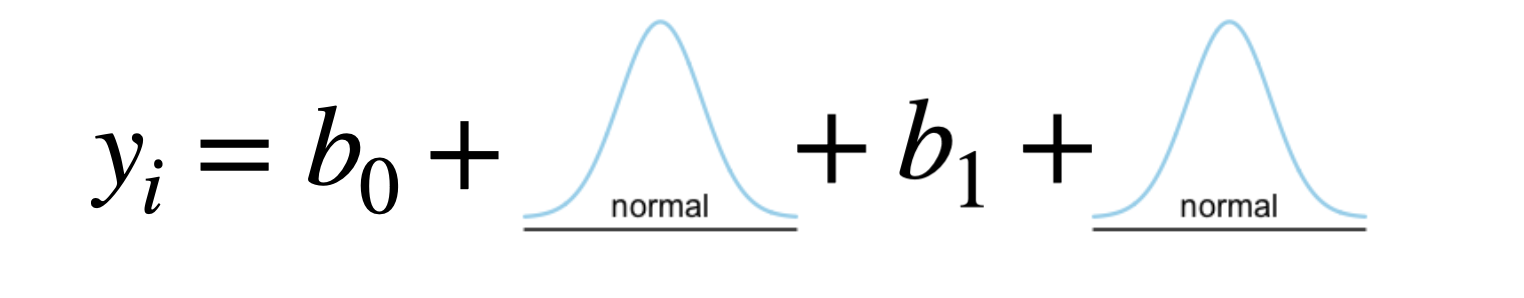
\includegraphics[keepaspectratio,width=12cm]{../images/14_design3/slide14_03.png}
\end{figure}

このように確率をふまえたモデルで考えると，群内計画のデータには2つの分布が混ざり込んでいるので，\keyterm{混合効果モデル}{こんごうこうかもでる}{Mixed Effect Model}と呼ぶことがあります。先ほどの群間計画では，$b_0+b_1$で平均値をずらした正規分布にデータが従うことになりましたが，群内計画では$b_0+b_1+d_i$が既に確率的に分布し，それが平均値となった確率分布がデータの従う分布になる，つまり(誤差の)正規分布の中に(個人差の)正規分布が入れ子になった形でモデルが表現されたことになります。分布が混ざったので\textbf{混合}というのですね。またより複雑なモデルの場合，この個人差を説明する他の変数や要因をつかって，個人差の分布もモデル化することになります。そのような場合，個人差に関係なく全体に及ぼす効果のことを\keyterm{固定効果}{こていこうか}{Fixed Effect}，個人差とともに変わりうる効果のことを\keyterm{変量効果}{へんりょうこうか}{Random Effect}と呼んで区別することがあります。名前だけでも覚えておいてください。


さて本講義はこの後，線形モデルに含まれる分布のことを考えながら，回帰係数や効果の大きさ，誤差の大きさを推定・評価していく\keyterm{推測統計学}{すいそくとうけいがく}{inferential statistics}へと展開していきます。
そのためにはデータがどのような分布をしているかを考え，理論的な分布の形に合わせて比較検討する，という手続きになります。具体的には「大体当てはまっている線形モデルの係数を考える」とか「線形モデルで計画された効果の大きさを推定する」「誤差の分布(散らばり)の大きさと効果の分布の大きさを比べる」といった手続きです。基本的にはこうした線形モデルであることを知っておいていただければ十分です。

また，統計モデルを使った推論は，どんどん発展させていくことができます。要因が1つ，2つと増えたように，混ぜ合わせる分布が複数あっても構わないのです。想像力を膨らませて，モデルにいろいろなパーツを組み立てることができるようになれば，心理学の研究や実験ももっとクリエイティブなものに感じられるでしょう。心理学の研究は，統計的な分析は，楽しいことなのですよ。




\section{課題}

\end{document}
